% overleaf的免費帳號不能邀請其他人共同編輯, 下面是我的推薦連結
% https://www.overleaf.com?r=cc96d36b&rm=d&rs=b
% 如果可以的話, 幫我增加一下點數 XD

% 如果需要更新, 請email至: wufish@gmail.com

\documentclass[12pt,a4paper,oneside]{book}  % NYCU碩論樣板

\linespread{2}

\usepackage[ top=2.5cm,bottom=2.5cm,left=3cm,right=2cm ]{ geometry }

%\documentclass[oneside,zh]{nctuthesis}
%\documentclass[conference]{IEEEtran}
%\documentclass[onecolumn, journal, 12pt]{IEEEtran}
%\documentclass[12pt,draftcls,onecolumn]{IEEEtran}
%\setlength{\baselineskip}{12.7pt}
\usepackage{subfigure}
%\usepackage{subcaption}
\usepackage{caption}
\usepackage{CJKutf8}
\usepackage{indentfirst}
\usepackage{array}
\usepackage{multirow}
\usepackage{amsthm}
\usepackage{amsmath}
\usepackage{amsfonts}
\usepackage{amssymb}
\usepackage{graphicx}
\usepackage{multirow}
\usepackage{setspace}
\usepackage{cite}
\usepackage{balance}
\usepackage{amssymb}
\usepackage{textcomp}
\usepackage{color}
\usepackage[ampersand]{easylist}
\ListProperties(Hide=100, Hang=true, Progressive=3ex, Style*=$\bullet$ ,
Style2*=\tiny$\blacksquare$ ,Style3*=$\circ$ ,Style4*=-- )
\usepackage{changepage}
%\usepackage{algorithmic}
\usepackage{algorithm}
\usepackage{algpseudocode}
\usepackage{graphics}
\usepackage{epsfig}
\floatname{algorithm}{Algorithm}
\renewcommand{\algorithmicrequire}{\textbf{Input:}}
\renewcommand{\algorithmicensure}{\textbf{Output:}}
\renewcommand{\algorithmiccomment}{// }
\usepackage{verbatim}
\newtheorem{theorem}{Theorem}
\newtheorem{lemma}{Lemma}
\newtheorem{prop}{Proposition}
\newtheorem{defn}{Definition}
\usepackage{array}
\usepackage{eqparbox}
\usepackage{textcomp}
\usepackage{amssymb}
\usepackage[T1]{fontenc}
\usepackage{enumerate}

\renewcommand*\rmdefault{ptm}
\usepackage[font={rm}]{caption}

\renewcommand\algorithmiccomment[1]{%
  \hfill\#\ \eqparbox{COMMENT}{#1}%
}
\usepackage{verbatim}

\usepackage{indentfirst}

\usepackage{chngcntr}
\counterwithout{figure}{chapter}
\counterwithout{table}{chapter}

\usepackage{color}
\usepackage{colortbl}
\newcommand{\textred}[1]{\textcolor{red}{#1}}
\newcommand{\textblue}[1]{\textcolor{blue}{#1}}
\newcommand{\textcyan}[1]{\textcolor{cyan}{#1}}
\newcommand{\myHuge}[1]{\fontsize{40}{50} #1}


% --------------------------------------------
% 在這邊寫自己的資料
\newcommand{\chineseTitle}{中文論文名字}
\newcommand{\englishTitle}{English Title}
\newcommand{\studentCnName}{學生名字}
\newcommand{\studentEnName}{XXXX Wu} % 書名頁
\newcommand{\studentEnNameA}{Wu, XXXX} % 封面用
% 英文名字有兩種寫法, 一個是姓在後, 一個是放前面. 

\newcommand{\advisorCnName}{指導教授}
\newcommand{\advisorEnName}{OOOO Tseng} % 書名頁
\newcommand{\advisorEnNameA}{Tseng, OOOO} % 封面用
\newcommand{\ThesisDate}{August 2022} % 碩論的日期
\newcommand{\ThesisDateTW}{中華民國~ 一一一年八月}

% --------------------------------------------


% source code hightlighting
\usepackage{listings}
\lstset{
	numbers=left,
	stepnumber=1,
	firstnumber=1,
	captionpos=b,
	tabsize=2,
	basicstyle=\small,
	numberfirstline=true
}

% setting the page number to footer
\usepackage{fancyhdr}
\fancyhf{}
\cfoot{\thepage}
\pagestyle{fancy}
% no header and footer bar
\renewcommand{\headrulewidth}{0pt}
\renewcommand{\footrulewidth}{0pt}

% line height setting
\linespread{1.5}
\usepackage{setspace}

\usepackage{background}
\newcommand\DeactivateBG{\backgroundsetup{contents={}}}
\newcommand\ActivateBG{
	\backgroundsetup{
		contents={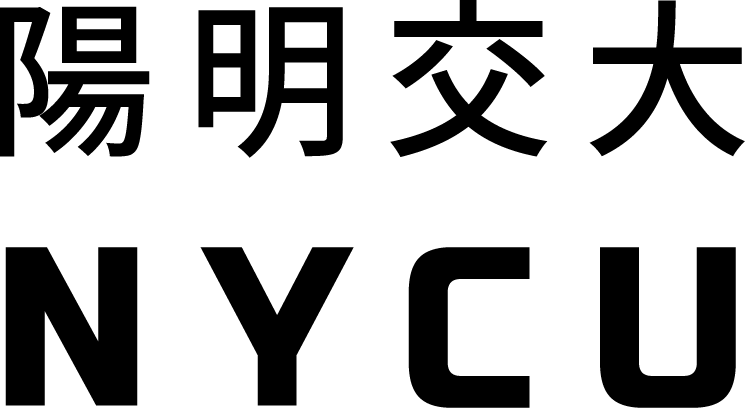
\includegraphics[]{Figures/logo.png}},
		scale=1,
		opacity=0.3,
		angle=0
	}
}



%%%%%%%%%%%%%%%%%%%%%%%%%%%%%% Textclass specific LaTeX commands.
%\newtheorem{theorem}{Theorem}
%\newtheorem{lemma}{Lemma}
%\newtheorem{prop}{Proposition}
%\newtheorem{defn}{Definition}

\usepackage{pdfpages}

%\doublespacing
\begin{document}


\DeactivateBG

%Cover
%\includepdf[pages={1},pagecommand={\thispagestyle{empty}}]{Andy_cover1.pdf}
%\includepdf[pages={1},pagecommand={\thispagestyle{empty}}]{Andy_cover2.pdf}

%審定書
%\includepdf[pages={1},pagecommand={\thispagestyle{empty}}]{auth_ch_Andy.pdf}
%\includepdf[pages={1},pagecommand={\thispagestyle{empty}}]{auth_en_Andy.pdf}

%授權書
%\includepdf[pages={1},pagecommand={\thispagestyle{empty}}]{auth_Andy.pdf}


\begin{CJK*}{UTF8}{bkai}


% =========================================================================
% 封面的設定, 像是日期之類的 settings for cover 
\newgeometry{top=3cm,bottom=3cm,left=3cm,right=3cm}

% 第一頁的封面, 記得修改系所


\begin{titlepage}

  \begin{center}
    \vspace{0.6cm}
    \fontsize{18}{22}\selectfont{國立陽明交通大學} \\
    \fontsize{18}{22}\selectfont{網路工程研究所} \\  
    \fontsize{18}{22}\selectfont{碩士論文}\\ 

    \vspace{1cm}
    
\fontsize{14}{17}\selectfont{Department of  xx} \\
\fontsize{16}{19}\selectfont{National Yang Ming Chiao Tung University} \\ 
\fontsize{16}{19}\selectfont{Master Thesis} \\ 

    \vspace{3.1cm}  
    \fontsize{18}{22}\selectfont \chineseTitle \\
    \fontsize{18}{22}\selectfont \englishTitle \\
    \vspace{3.1cm}
        
    \fontsize{18}{22}\selectfont 研究生: {\studentCnName}  (\studentEnNameA) \\
    \fontsize{18}{22}\selectfont 指導教授: {\advisorCnName} (\advisorEnNameA) \\
    
    \vspace{\fill}
    
    \fontsize{18}{22}\selectfont \ThesisDateTW \\
    \fontsize{18}{22}\selectfont \ThesisDate
    
  \end{center}

\end{titlepage}

% 第二頁的書名頁, 記得修改系所, 日期
\begin{titlepage}
  \begin{center}
    \LARGE \chineseTitle \\
    \LARGE \englishTitle \\
  
    \vspace{1.5cm}
  
    \fontsize{14}{14}\selectfont{
    \begin{tabular}{r l c r l}
    研究生: & \studentCnName & \hspace{1.5cm} & Student: & \studentEnName \\
    指導教授: & \advisorCnName ~ 博士 & \hspace{1.5cm} & Advisor: & Dr. \advisorEnName \\
    \end{tabular}
    }
    
    \vspace{1.5cm}

    \fontsize{14}{17}\selectfont{國立陽明交通大學} \\
    \fontsize{14}{17}\selectfont{網路工程研究所} \\  
    \fontsize{14}{17}\selectfont{碩士論文}\\     
    
    \vspace{2cm}

    \fontsize{14}{14}\selectfont{
    A Thesis \\
    Submitted to Institute of Computer Science and Engineering \\
    College of Computer Science \\
    National Yang Ming Chiao Tung University \\
    in partial Fulfillment of the Requirements \\
	for the Degree of \\
    Master \\
	in  \\
	Computer Science \\
    }
    
    \vspace{\fill}

    \ThesisDate \\
    Taiwan, Republic of China \\
    ~ \\

    \fontsize{18}{22}\selectfont  \ThesisDateTW


  \end{center}
\end{titlepage}



% 博士論文版的封面&書名頁


\begin{titlepage}

  \begin{center}
    \vspace{0.6cm}
    \fontsize{18}{22}\selectfont{國立陽明交通大學} \\
    \fontsize{18}{22}\selectfont{網路工程研究所} \\  
    \fontsize{18}{22}\selectfont{博士論文}\\ 

    \vspace{1cm}
    
\fontsize{14}{17}\selectfont{Department of  xx} \\
\fontsize{16}{19}\selectfont{National Yang Ming Chiao Tung University} \\ 
\fontsize{16}{19}\selectfont{Doctoral Dissertation} \\ 

    \vspace{3.1cm}  
    \fontsize{18}{22}\selectfont \chineseTitle \\
    \fontsize{18}{22}\selectfont \englishTitle \\
    \vspace{3.1cm}
        
    \fontsize{18}{22}\selectfont 研究生: {\studentCnName}  (\studentEnNameA) \\
    \fontsize{18}{22}\selectfont 指導教授: {\advisorCnName} (\advisorEnNameA) \\
    
    \vspace{\fill}
    
    \fontsize{18}{22}\selectfont \ThesisDateTW \\
    \fontsize{18}{22}\selectfont \ThesisDate
    
  \end{center}

\end{titlepage}
\begin{titlepage}
  \begin{center}
    \LARGE \chineseTitle \\
    \LARGE \englishTitle \\
  
    \vspace{1.5cm}
  
    \fontsize{14}{14}\selectfont{
    \begin{tabular}{r l c r l}
    研究生: & \studentCnName & \hspace{1.5cm} & Student: & \studentEnName \\
    指導教授: & \advisorCnName ~ 博士 & \hspace{1.5cm} & Advisor: & Dr. \advisorEnName \\
    \end{tabular}
    }
    
    \vspace{1.5cm}

    \fontsize{14}{17}\selectfont{國立陽明交通大學} \\
    \fontsize{14}{17}\selectfont{網路工程研究所} \\  
    \fontsize{14}{17}\selectfont{博士論文}\\     
    
    \vspace{2cm}

    \fontsize{14}{14}\selectfont{
    A Dissertation \\
    Submitted to Institute of Computer Science and Engineering \\
    College of Computer Science \\
    National Yang Ming Chiao Tung University \\
    in partial Fulfillment of the Requirements \\
	for the Degree of \\
    Doctor of Philosoph \\
	in  \\
	Computer Science \\
    }
    
    \vspace{\fill}

    \ThesisDate \\
    Taiwan, Republic of China \\
    ~ \\

    \fontsize{18}{22}\selectfont  \ThesisDateTW


  \end{center}
\end{titlepage}




\restoregeometry
% =========================================================================

% 加入浮水印
\ActivateBG

\frontmatter
\pagenumbering{roman}
{\fontfamily{ptm}\selectfont


% =========================================================================
% 中英文摘要 chinese and english abstract
\addcontentsline{toc}{chapter}{摘\,\,\,\,\,要} 
  \begin{center}
	\large
    \begin{singlespace}    
      \textbf{\chineseTitle{}} \\[0.5cm]
    \end{singlespace}
    
    \begin{singlespace}    

    	學生      :\studentCnName{}  \hspace{2.5cm}  指導教授  :\advisorCnName \hspace{0.1cm} 博士 \\
         [0.5cm]

    \end{singlespace}
    

    國立陽明交通大學網路工程研究所碩士班 \\[0.5cm]
    \makebox[4em][s]{\textbf{摘要}} \\[0.5cm]
    	
  \end{center}
  \normalsize 
  \hspace{0.75cm} 在日常生活中,重要區域有安全監控的需求.......

  \vspace{1cm}

  % 中文摘要及關鍵詞 5-7 個 
  \textbf{關鍵字:}光達, 資料融合, 物聯網, 穿戴式計算, 身分識別
 \newpage
\addcontentsline{toc}{chapter}{Abstract}  \begin{center}
  	\large
  	\begin{singlespace}
  		\textbf{\englishTitle{}} \\[0.5cm]
  	\end{singlespace}
  	
  	\begin{singlespace}

  			Student : \studentEnName{}  \hspace{1.0cm} Advisor  : Dr.\, \advisorEnName \\
  			[0.5cm]

  	\end{singlespace}
  	
  	\begin{singlespace}
  		Institute of Network Engineering\\ National Yang Ming Chiao Tung University\\[0.5cm]
  	\end{singlespace}
  	\textbf{Abstract} \\[0.5cm]
  	
  \end{center}
  \normalsize 
  
%  \hspace{0.25cm}
Surveillance has been widely used for security and management purposes. Through computer vision technologies, we can capture human .......


\vspace{1cm}

% 5-7 Keywords (English) 
\textbf{Keywords: Data Fusion, IoT, LiDAR, Surveillance, Wearable Computing.} 
  
 \newpage

% 致謝 Acknowledgement
\addcontentsline{toc}{chapter}{誌\,\,\,\,\,謝} 
% --- Acknowledgment ---
\begin{CJK*}{UTF8}{bkai}
\begin{center}
\Large
\textbf{誌~~~~~~謝}
\end{center}

\vspace{1cm}
\linespread{2}%
\selectfont
\hspace{0.25cm}

謝天謝地

\vspace{3cm}
\begin{flushright}
XXXXX 於

國立交通大學網路工程研究所碩士班

中華民國 \, 108 年 \, 8 \,月
\end{flushright}
\end{CJK*}
\newpage
% =========================================================================

\addcontentsline{toc}{chapter}{Contents} \tableofcontents \newpage
\renewcommand{\numberline}[1]{Figure~#1\hspace*{1em}}
\addcontentsline{toc}{chapter}{List of Figures} \listoffigures \newpage
\renewcommand{\numberline}[1]{Table~#1\hspace*{1em}}
%\addcontentsline{toc}{chapter}{List of Tables} \listoftables \newpage

\mainmatter
\pagenumbering{arabic} % enabling page numbering

% =========================================================================
% 論文的內文, 可以每個章節一個.tex檔案 (put your statements in the following)
\chapter{Introduction}
\label{ch:intro}
Video-based surveillance systems have been widely used in places such as plaza, office, factory, hotel, and conference hall for security purposes\cite{collins2000system},\cite{wang2013intelligent}. ......

The rest of this paper is organized as follows. Chapter 2 reviews some related work. Chapter 3 introduces our system architecture. Chapter 4 explains the details of our pairing algorithm. Performance evaluation results are in Chapter 5. Conclusions are in Chapter 6.
 \newpage
\chapter{Related Work}
\label{ch:relatedwork}
The PID issue has been widely studied in the field of computer vision and IoT by using various devices. In the field of computer vision, camera is the most popular device. Face recognition technologies are surveyed in \cite{zhao2003face}. Reference \cite{parkhi2015deep} focuses on how to collect a very large training dataset and build a very deep CNN model for face recognition, but training process is extremely computationally expensive. A hybrid RFID and computer vision system for localization and tracking of RFID tags is proposed in \cite{goller2014fusing}. Reference \cite{isasi2010location} presents a solution which combines RFID with object tracking through cameras. Reference \cite{germa2010vision} presents a fusion system consisting of an RFID reader and a camera crew on a mobile robot platform to track people. These works \cite{goller2014fusing},\cite{isasi2010location},\cite{germa2010vision} fuse data from camera and RFID, but their accuracy highly depends on the density of RFID antennas. Thus, they are not suitable for longer range PID. Reference \cite{munaro2014fast} proposes a fast multi-people tracking algorithm for service robots through RGB-D camera. In \cite{spinello2011people}, people detection is realized by dense depth data, called Histogram of Oriented Depths (HOD).  \newpage
\chapter{System Model}
\label{ch:architecture}

Our goal is to .... \newpage
\chapter{Data Fusion Algorithm}
\label{ch:method}

\begin{figure}[htb]
	\centering
	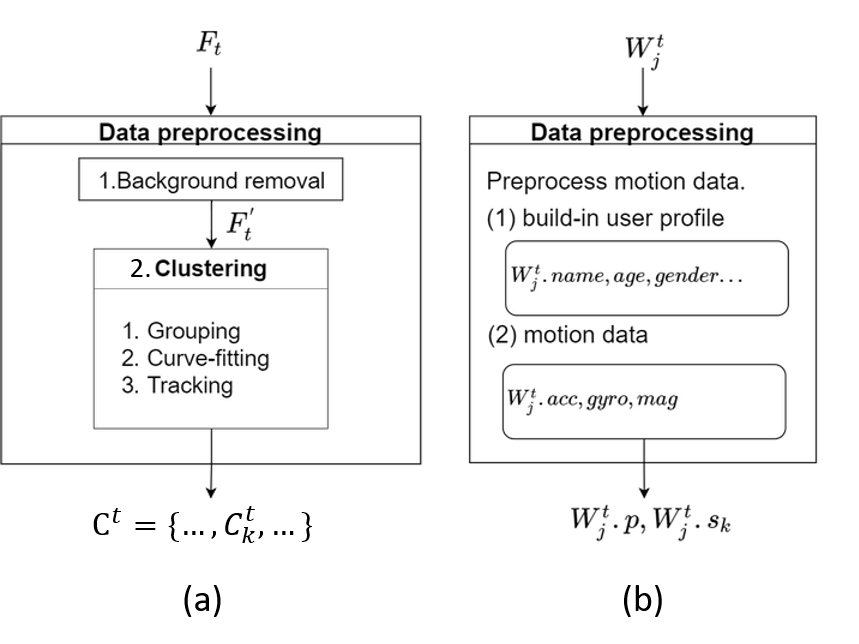
\includegraphics[width=0.6\textwidth]{img/data_preprocessing.png}
	\caption{Data preprocessing}
	\label{fig:model}
	\vspace{-10mm}
\end{figure}

\section{Data Preprocessing}
\label{sec:SMA}
Both LiDAR and wearable sensors will generate continuous data to our fusion server. Fig~\ref{fig:model} shows how these raw data are preprocessed. 


\subsection{2D LiDAR Data}
 The LiDAR data preprocessing contains two parts: (i) background removal and (ii) clustering. Background removal 
....

 \newpage
\chapter{Performance Evaluation}
\label{ch:evaluation}

\vspace{-5mm}

In this section, ....
 \newpage
\chapter{Conclusions}
\label{ch:conclusion}
Although LiDAR has been applied .......
 
 \newpage
% =========================================================================


% =========================================================================
% 參考文獻的檔案 Reference file: ref.bib
% ref的寫法可以參考這邊: https://hackmd.io/Bc1-FIIISka6DW15sPprAw
\addcontentsline{toc}{chapter}{Bibliography}
\bibliographystyle{IEEEtran}
\bibliography{ref}
}
% =========================================================================


\end{CJK*}
\balance

\end{document}



